\documentclass[tikz,border=5pt]{standalone}
\usepackage{amssymb,amsmath}
\newcommand{\C}{\mathbb{C}}
\begin{document}
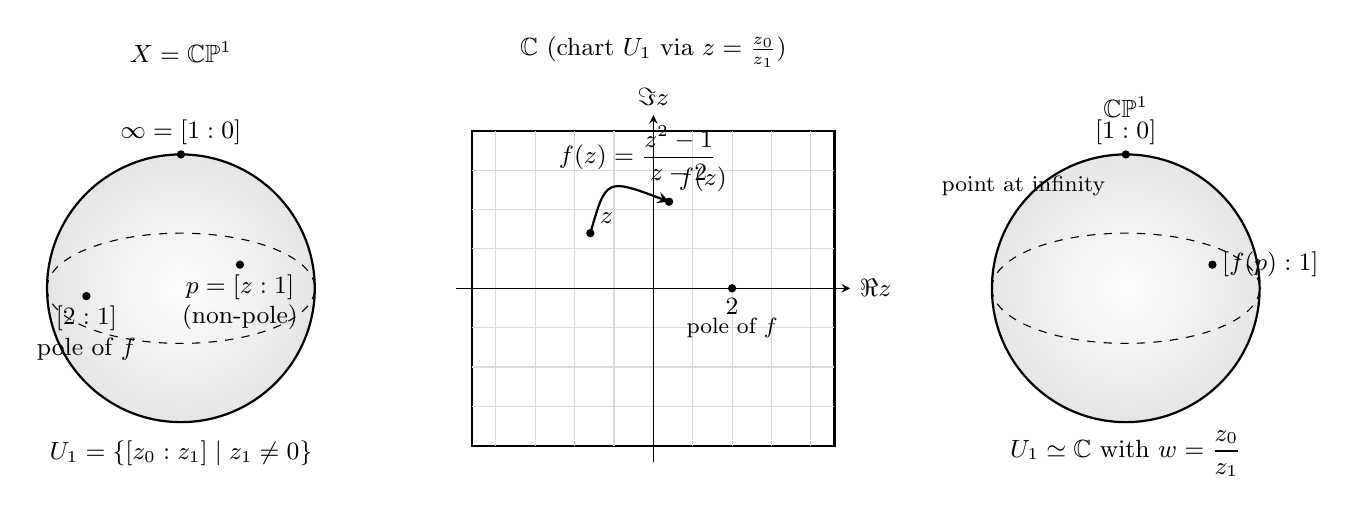
\begin{tikzpicture}[font=\small,>=stealth]
%========================================
% LEFT: Domain CP^1 with affine charts
%========================================
\begin{scope}[shift={(-6,0)}]
	% Sphere = CP^1
	\shade[inner color=white, outer color=gray!20, draw=black, thick]
	(0,0) circle (1.7);
	\node at (0,3) {$X=\mathbb{CP}^1$};
	% North pole = infinity [1:0]
	\fill (0,1.7) circle (1.5pt);
	\node[above] at (0,1.7) {$\infty=[1:0]$};
	% Equator: affine chart U_1
	\draw[dashed] (-1.7,0) arc (180:360:1.7 and 0.7);
	\draw[dashed] (-1.7,0) arc (180:0:1.7 and 0.7);
	\node at (0,-2.1) {$U_1=\{[z_0:z_1]\mid z_1\neq 0\}$};
%	\node at (0,-2.6) {\footnotesize coord.\ $z=\dfrac{z_0}{z_1}$};
	% Mark a non-pole p=[z:1]
	\fill (.75,0.3) circle (1.5pt)
	node[below, align=center] {$p=[z:1]$\\ (non-pole)};
	% Mark a pole point [2:1] on equator
	\fill (-1.2,-0.1) circle (1.5pt)
	node[below, align=center] {$[2:1]$\\ pole of $f$};
%	% Tiny label for upper chart U_0
%	\node at (0,1.0) {\footnotesize $U_0:\ u=\dfrac{z_1}{z_0}$};
\end{scope}
%========================================
% MIDDLE: Affine chart C with rational f
%========================================
\begin{scope}
	% Rectangle for C
	\draw[thick] (-2.3,-2.0) rectangle (2.3,2.0);
	\node at (0,3) {$\mathbb{C}$ (chart $U_1$ via $z=\frac{z_0}{z_1}$)};
	% Grid
	\foreach \x in {-2,-1.5,...,2}
	\draw[gray!30] (\x,-2.0) -- (\x,2.0);
	\foreach \y in {-1.5,-1,...,1.5}
	\draw[gray!30] (-2.3,\y) -- (2.3,\y);
	% Axes
	\draw[->] (-2.5,0) -- (2.5,0) node[right] {$\Re z$};
	\draw[->] (0,-2.2) -- (0,2.2) node[above] {$\Im z$};
	% Mark z=p and z=2
	\fill (-0.8,0.7) circle (1.5pt);
	\node[above right] at (-0.8,0.7) {$z$};
	\fill (1,0) circle (1.5pt)
	node[below] {$2$};
	\node at (1,-0.5) {\footnotesize pole of $f$};
	% Image f(z)
	\fill (0.2,1.1) circle (1.5pt);
	\node[above right] at (0.2,1.1) {$f(z)$};
	% Sketch: arrow showing f
	\draw[->,thick]
	(-0.8,0.7) .. controls (-0.6,1.4) .. (0.2,1.1);
	\node at (-0.2,1.7) {$f(z)=\dfrac{z^2-1}{z-2}$};
%	% Indication that f(z) blows up near 2 (pole)
%	\draw[->,densely dashed]
%	(1.4,0.9) -- (2.0,1.7);
%	\node at (2.2,1.9) {\footnotesize ``$\infty$''};
\end{scope}

%========================================
% RIGHT: Target CP^1 (Riemann sphere)
%========================================
\begin{scope}[shift={(6,0)}]
	% Sphere = CP^1
	\shade[inner color=white, outer color=gray!20, draw=black, thick]
	(0,0) circle (1.7);
	\node at (0,2.3) {$\mathbb{CP}^1$};
	
	% North pole = [1:0]
	\fill (0,1.7) circle (1.5pt);
	\node[above] at (0,1.7) {$[1:0]$};
	\node at (-1.3,1.3) {\footnotesize point at infinity};
	
	% Equator (affine chart U_1 of target)
	\draw[dashed] (-1.7,0) arc (180:360:1.7 and 0.7);
	\draw[dashed] (-1.7,0) arc (180:0:1.7 and 0.7);
	\node at (0,-2.1) {$U_1\simeq\C$ with $w=\dfrac{z_0}{z_1}$};
	
	% Image of a non-pole p: [f(p):1]
	\fill (1.1,0.3) circle (1.5pt);
	\node[right] at (1.1,0.3) {$[f(p):1]$};
	
	% Image of pole: [1:0]
	% (arrow shown below)
\end{scope}

%%========================================
%% ARROWS: charts, f, F
%%========================================
%
%% Chart phi_1: U_1 -> C (domain)
%\draw[->,thick]
%(-4,0.2) .. controls (-2.5,1.7) .. (-0.4,1.4);
%\node at (-2.7,2.0) {$\phi_1([z_0:z_1])=\dfrac{z_0}{z_1}$};
%
%% Inclusion i: C -> CP^1 (target affine chart)
%\draw[->,thick]
%(2.4,-0.2) .. controls (3.7,-1.3) .. (5.5,-0.4);
%\node at (4.0,-1.5) {$i(w)=[w:1]$};
%
%% Big arrow: F: CP^1 -> CP^1
%\draw[->,thick]
%(-4.0,0.3) .. controls (0,3.0) .. (4.0,0.3);
%\node at (0,3.3) {$F$};
%
%% Arrow showing F(p) via chart: p -> f(p) -> [f(p):1]
%\draw[->,thick]
%(-4.0,0.3) .. controls (-2.0,0.9) .. (-0.8,0.8); % p to z
%\draw[->,thick]
%(-0.8,0.8) .. controls (0.0,1.6) .. (0.2,1.1);   % z to f(z)
%\draw[->,thick]
%(0.2,1.1) .. controls (3.3,1.7) .. (5.0,0.4);    % f(z) to [f(z):1]
%\node at (0.0,2.2) {\footnotesize $p\mapsto f(p)\mapsto [f(p):1]$};
%
%% Arrow showing pole [2:1] -> [1:0]
%\draw[->,thick]
%(-4.8,-0.1) .. controls (-1.8,-2.2) .. (5.0,1.7);
%\node at (0.2,-2.4) {\footnotesize $[2:1]\mapsto [1:0]$ (pole $\mapsto$ infinity)};

\end{tikzpicture}
\end{document}